\chapter{Практическая часть}
\label{ch:practice}

\section{Установка Ansible на gateway}

Ansible устанавливается через \texttt{pip3} — это обеспечивает актуальную
версию, независимую от пакетной базы Ubuntu~20.04:

\begin{lstlisting}
apt-get install -y python3 python3-pip openssh-client sshpass
pip3 install ansible
\end{lstlisting}

Проверка установки:
\begin{lstlisting}
ansible --version
\end{lstlisting}

% --- Скриншот: ansible --version ---
\begin{figure}[h]
  \centering
  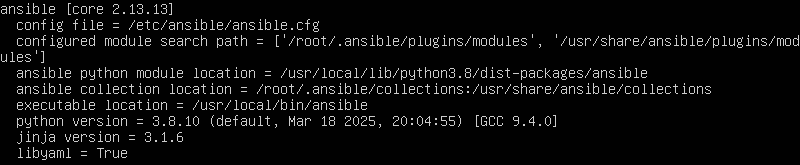
\includegraphics{img/05_ansible_version}
  \caption{Вывод \texttt{ansible -{}-version} — Ansible успешно установлен}
  \label{fig:ansible_version}
\end{figure}

\section{Генерация SSH-ключа}

На \texttt{gateway} генерируется ключ \texttt{ed25519} без пароля
(пустой passphrase позволяет Ansible подключаться без интерактивного ввода):

\begin{lstlisting}
ssh-keygen -t ed25519 -a 100
\end{lstlisting}

При запросе имени файла нажимаем Enter (путь по умолчанию:
\texttt{\textasciitilde/.ssh/id\_ed25519}).
При запросе пароля — Enter дважды (пустой пароль).

% --- Скриншот: вывод ssh-keygen ---
\begin{figure}[h]
  \centering
  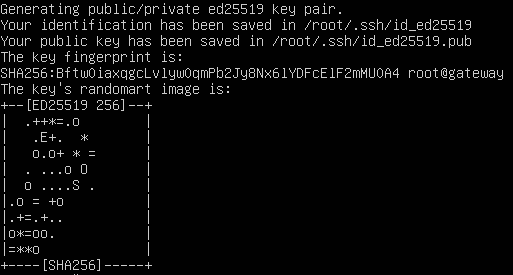
\includegraphics{img/06_ssh_keygen}
  \caption{Генерация SSH-ключа \texttt{ed25519} на \texttt{gateway}}
  \label{fig:ssh_keygen}
\end{figure}

\section{Копирование SSH-ключа на клиентов}

Публичный ключ копируется на каждую клиентскую ВМ командой \texttt{ssh-copy-id}.
Скрипт запрашивает пароль пользователя клиента:

\begin{lstlisting}
ssh-copy-id -i ~/.ssh/id_ed25519.pub username@192.168.29.10
ssh-copy-id -i ~/.ssh/id_ed25519.pub username@192.168.29.6
\end{lstlisting}

Ожидаемый вывод после каждой команды:
\begin{lstlisting}
Number of key(s) added: 1
\end{lstlisting}

% --- Скриншот: ssh-copy-id на desktop1 (Number of key(s) added: 1) ---
\begin{figure}[h]
  \centering
  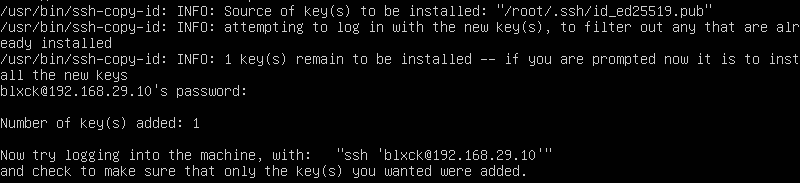
\includegraphics{img/07_ssh_copy_desktop}
  \caption{Копирование SSH-ключа на \texttt{desktop1}}
  \label{fig:ssh_copy_desktop}
\end{figure}

% --- Скриншот: ssh-copy-id на wordpress (Number of key(s) added: 1) ---
\begin{figure}[h]
  \centering
  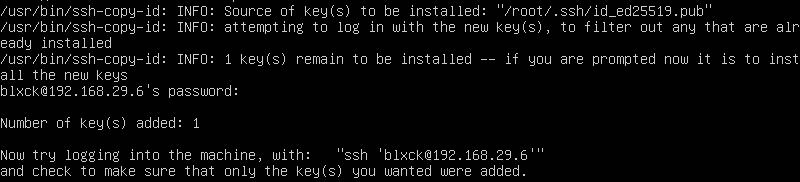
\includegraphics{img/08_ssh_copy_wordpress}
  \caption{Копирование SSH-ключа на \texttt{wordpress}}
  \label{fig:ssh_copy_wordpress}
\end{figure}

\section{Создание структуры Ansible}

\subsection{Инвентарный файл hosts}

Файл \texttt{/etc/ansible/hosts} описывает группу \texttt{clients}
с двумя управляемыми узлами:

\begin{lstlisting}
[clients]
desktop1  ansible_host=192.168.29.10  ansible_user=username
wordpress ansible_host=192.168.29.6   ansible_user=username
\end{lstlisting}

% --- Скриншот: cat /etc/ansible/hosts ---
\begin{figure}[h]
  \centering
  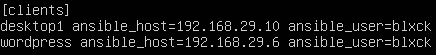
\includegraphics{img/09_ansible_hosts}
  \caption{Содержимое файла \texttt{/etc/ansible/hosts}}
  \label{fig:ansible_hosts}
\end{figure}

\subsection{Файл конфигурации ansible.cfg}

Файл \texttt{/etc/ansible/ansible.cfg} задаёт путь к inventory и отключает
проверку host~key (допустимо в учебной среде):

\begin{lstlisting}
[defaults]
inventory        = /etc/ansible/hosts
host_key_checking = False
\end{lstlisting}

\subsection{Проверка подключения — ansible ping}

\begin{lstlisting}
ansible clients -m ping
\end{lstlisting}

Ожидаемый вывод:
\begin{lstlisting}
desktop1  | SUCCESS => {"ping": "pong"}
wordpress | SUCCESS => {"ping": "pong"}
\end{lstlisting}

% --- Скриншот: ansible clients -m ping (SUCCESS) ---
\begin{figure}[h]
  \centering
  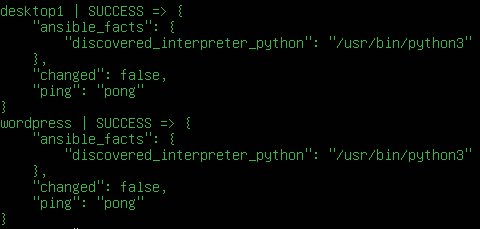
\includegraphics{img/10_ansible_ping}
  \caption{Проверка связности Ansible с клиентами}
  \label{fig:ansible_ping}
\end{figure}

\section{Плейбук monitoring.yml}

Плейбук создаётся по пути\\ \texttt{/etc/ansible/playbooks/monitoring.yml}.\\
\\Задачи плейбука:

\begin{enumerate}
  \item Создать директорию \texttt{/etc/ansible/monitoring/} на control node
        (\texttt{delegate\_to: localhost}, \texttt{run\_once: true});
  \item Вычислить свободное место на разделе \texttt{/} клиента
        через \texttt{set\_fact} и фильтры Jinja2;
  \item Сохранить файл \texttt{inventory\_hostname\_info.txt} с данными
        клиента на control node (\texttt{delegate\_to: localhost}).
\end{enumerate}

\begin{lstlisting}
---
- name: collect info to server
  hosts: clients
  gather_facts: true

  tasks:
    - name: create monitoring directory
      file:
        path: /etc/ansible/monitoring
        state: directory
        mode: '0755'
      delegate_to: localhost
      run_once: true

    - name: get free space in root partition
      set_fact:
        root_free_space_gb: >-
          {{ ( ansible_mounts
               | selectattr('mount', 'equalto', '/')
               | map(attribute='size_available')
               | first | float / 1024 / 1024 / 1024
             ) | round(2) }}

    - name: save info file to server
      copy:
        dest: "/etc/ansible/monitoring/{{ inventory_hostname }}_info.txt"
        content: |
          Hostname: {{ ansible_hostname }}
          IP: {{ ansible_default_ipv4.address }}
          OS: {{ ansible_distribution }} {{ ansible_distribution_version }}
          Free disk space on /: {{ root_free_space_gb }} GB
        mode: '0644'
      delegate_to: localhost
\end{lstlisting}

% --- Скриншот: cat /etc/ansible/playbooks/monitoring.yml ---
\begin{figure}[h]
  \centering
  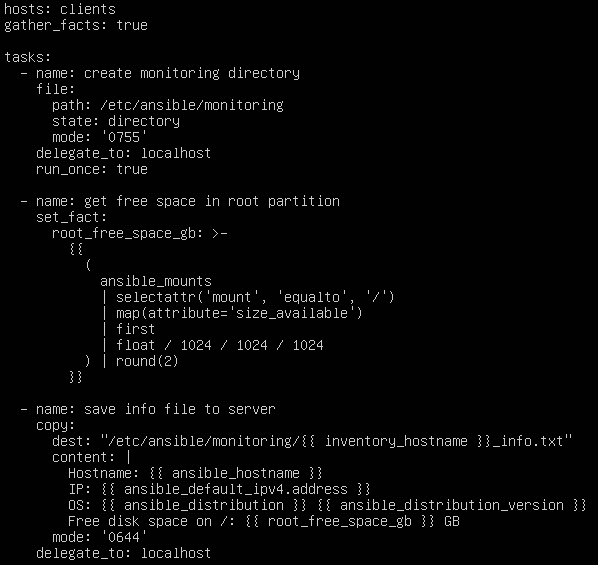
\includegraphics{img/11_playbook_content}
  \caption{Содержимое плейбука \texttt{monitoring.yml}}
  \label{fig:playbook_content}
\end{figure}

\section{Запуск плейбука и результаты}

Плейбук запускается командой:
\begin{lstlisting}
ansible-playbook /etc/ansible/playbooks/monitoring.yml
\end{lstlisting}

% --- Скриншот: вывод ansible-playbook (ok, changed, failed=0) ---
\begin{figure}[h]
  \centering
  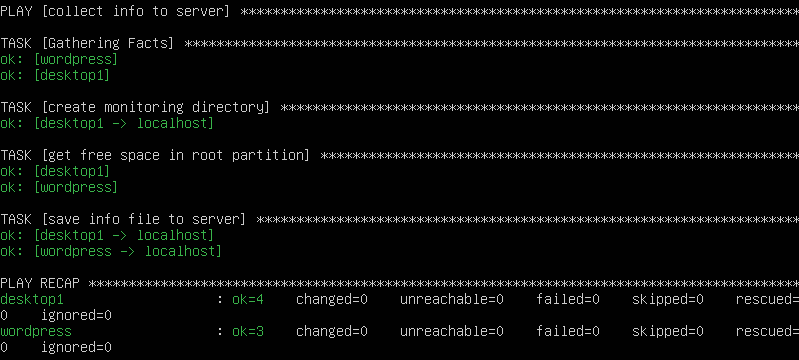
\includegraphics{img/12_playbook_run}
  \caption{Вывод выполнения плейбука — \texttt{failed=0}}
  \label{fig:playbook_run}
\end{figure}

\subsection{Проверка собранных данных}

После выполнения плейбука в директории\\ \texttt{/etc/ansible/monitoring/}
появляются два файла. Содержимое проверяется командой \texttt{cat}:

\begin{lstlisting}
cat /etc/ansible/monitoring/desktop1_info.txt
cat /etc/ansible/monitoring/wordpress_info.txt
\end{lstlisting}

% --- Скриншот: cat desktop1_info.txt ---
\begin{figure}[h]
  \centering
  
\includegraphics{img/13_info_desktop1}
  \caption{Данные мониторинга клиента \texttt{desktop1}}
  \label{fig:info_desktop1}
\end{figure}

% --- Скриншот: cat wordpress_info.txt ---
\begin{figure}[h]
  \centering
  
\includegraphics{img/14_info_wordpress}
  \caption{Данные мониторинга клиента \texttt{wordpress}}
  \label{fig:info_wordpress}
\end{figure}

\endinput
